\chapter{\textit{Introduction}}
\section{Previous Requirements}
The minimum requirements to run properly the application are:
\begin{itemize} \itemsep0pt \parskip0pt \parsep0pt
	\renewcommand{\labelitemi}{$\rightarrow$}
	\item Operative System: Mac OS X, Windows (XP or newer), Linux, Solaris. 32 or 64 bits architectures.
	\item Software: Java 8 (mandatory requirement).
	\item CPU: AMD or Intel {$>$} 1Ghz.
	\item Memory: At least 512Mb availables.
	\item Graphics Card: AMD/ATI Radeon 9500, NVIDIA GeForce 5 FX, Intel GMA 4500, or better.
	\item Screen: minimun resolution 1024x768
\end{itemize}
\newpage

\section{Application Run}
To run the application it's necessary have installed at least the version 8 of the \textit{Java Virtual Machine} (\emph{http://www.java.com/en/download/}).\\
According to the Operative System installed, can run the application directly from the file explorer or through the system console writing:\\ \emph{java -jar jtlc.jar} over the application folder.
When the application start a new file (\textit{jtlc.settings.props}) is created to store the current settings.
In picture \ref{fig:inicial} is detailed  the application main window.

\begin{figure}[H]
	\vspace{0cm}
	\centering
	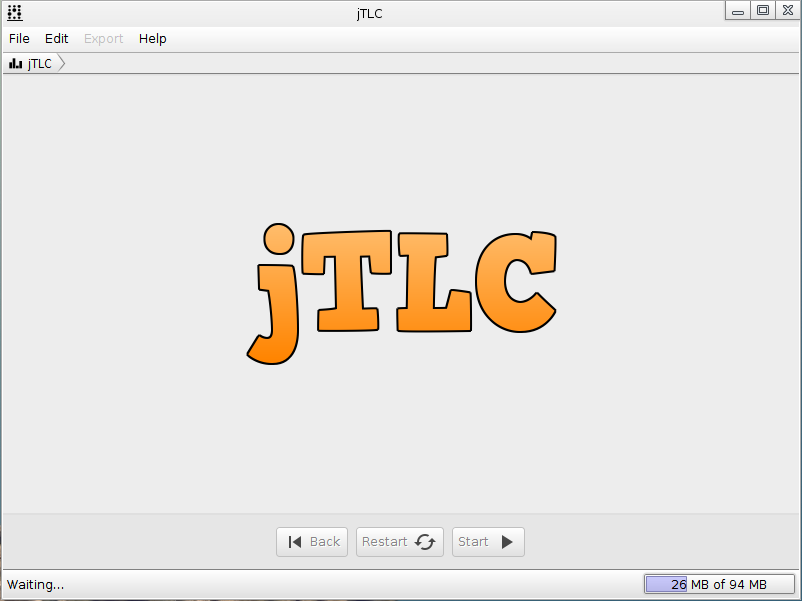
\includegraphics[width=385px]{imagenes/main}
	\centering
	\vspace{-0.4cm}
	\caption{Application initial screen.}
	\label{fig:inicial}
	\vspace{-0.25cm}
\end{figure}
\newpage

\section{Application Settings}
The application settings allows to the user change the system language, projects workspace and enable or disable animations (like screen transition between each analysis screen). To access the settings screen go to \emph{Edit} \ding{222} \emph{Change settings} on the main menu bar.
In the settings screen use \emph{Directory Selector} to change current workspace, the language select to change the application languge, move the animations switch to enable or disable animations. To save current settings click on the button Accept or press \emph{Enter} key from your keyboard. to discard the current settings click on the button Cancel or press \emph{Esc} key.

\begin{figure}[H]
	\vspace{0cm}
	\centering
	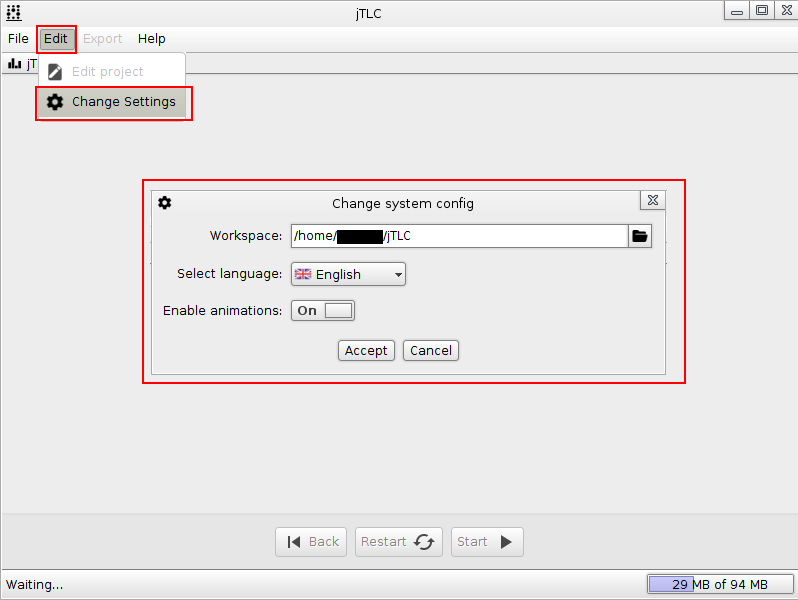
\includegraphics[width=385px]{imagenes/settings}
	\centering
	\vspace{-0.4cm}
	\caption{Application settings.}
	\label{fig:settings}
	\vspace{-0.25cm}
\end{figure}
\newpage

\chapter{\textit{Projects}}
\section*{Start new project}
To start analyzing samples first is necessary start a new project. In the \emph{File} menu use the option \emph{New Project} to create a new project, then the \emph{Create a new Project} dialog will be shown. In this dialog you can introduce the basic information of the project. Click on \emph{Accept} to continue or \emph{Cancel} to abort.
\begin{figure}[H]
	\vspace{0cm}
	\centering
	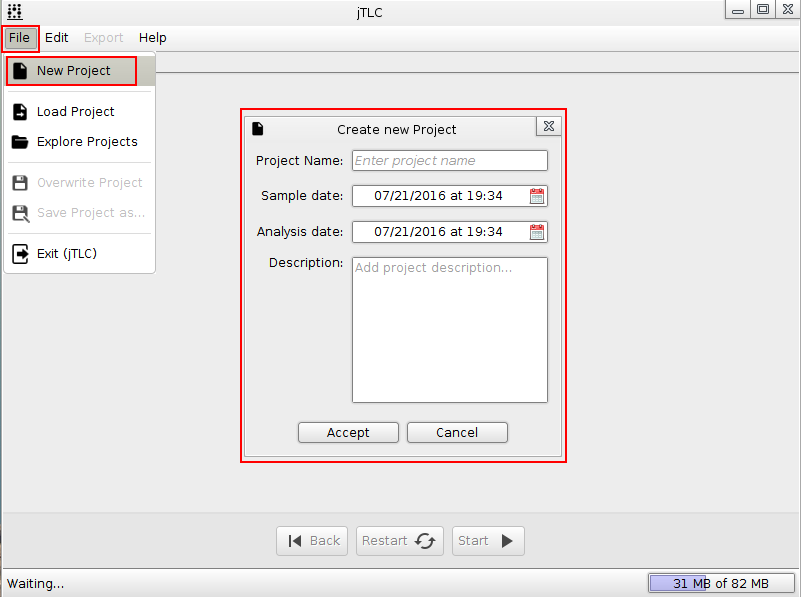
\includegraphics[width=385px]{imagenes/new_project}
	\centering
	\vspace{-0.4cm}
	\caption{New project menu.}
	\label{fig:new_project}
	\vspace{-0.25cm}
\end{figure}
\newpage

\section{Load existent project}
To load a previous project use the option \emph{Load Project} in the \emph{File} menu. A file chooser will be shown where you can select a \textit{jTLC} project file with extension \emph{.jtlc}, select the file and click on \emph{Open} to load or \emph{Cancel} to abort.
\begin{figure}[H]
	\vspace{0cm}
	\centering
	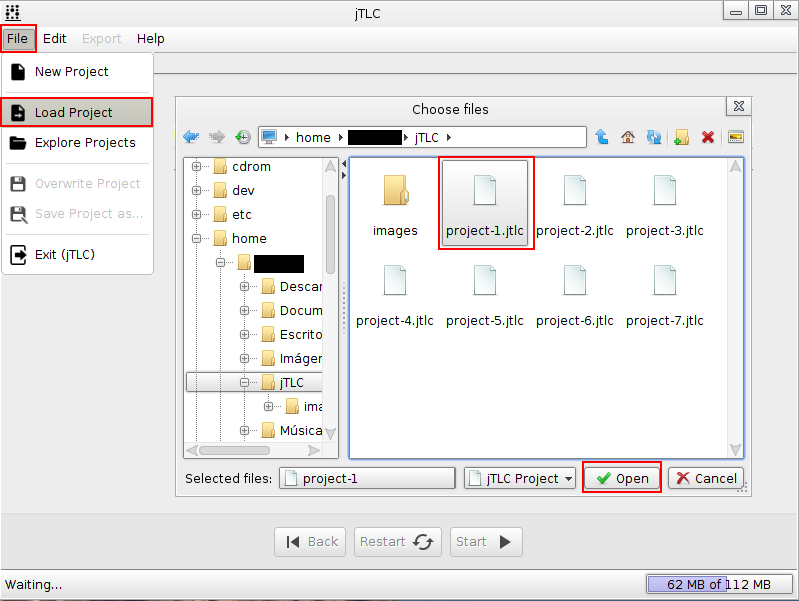
\includegraphics[width=385px]{imagenes/load_project}
	\centering
	\vspace{-0.4cm}
	\caption{New project menu.}
	\label{fig:load_project}
	\vspace{-0.25cm}
\end{figure}
\newpage

\section{Explore projects}
To explore old projects use the option \emph{Explore Projects} in the \emph{File} menu. A directory chooser will be shown where you can select a folder with the \textit{jTLC} project files (\emph{.jtlc} extension), select the folder and click on \emph{Choose} to explore projects or \emph{Cancel} to abort.
\begin{figure}[H]
	\vspace{0cm}
	\centering
	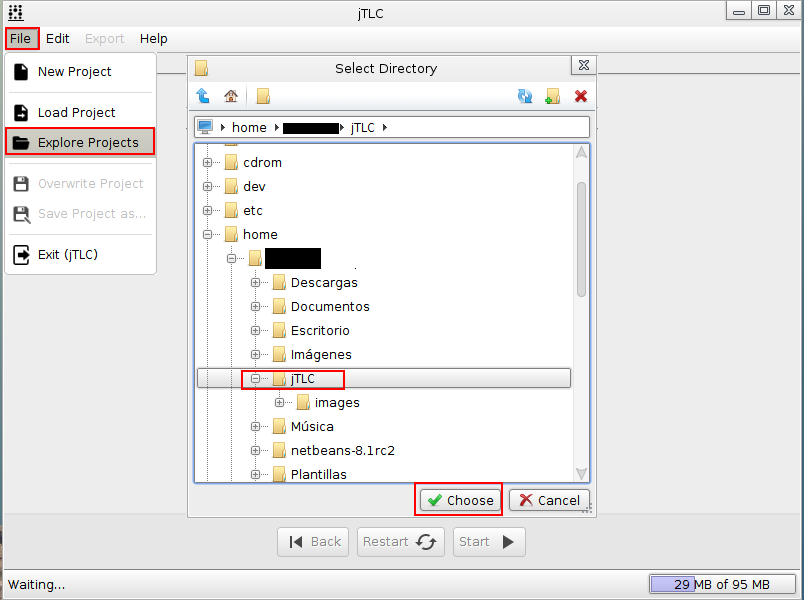
\includegraphics[width=385px]{imagenes/explore_projects}
	\centering
	\vspace{-0.4cm}
	\caption{Explore projects.}
	\label{fig:explore_projects}
	\vspace{-0.25cm}
\end{figure}
\newpage

\subsection{Project Gallery}
After select a folder to explore, the \emph{Project Gallery} will be shown where all the projects in the selected folder are displayed. To view the project details do a click over the project image, the project will be selected as the current project. Use the \emph{arrow keys} Left and Right or use the mouse \emph{scroll wheel} to travel between projects. When a project was selected click on the button \emph{Start} to continue working on that project.
\begin{figure}[H]
	\vspace{0cm}
	\centering
	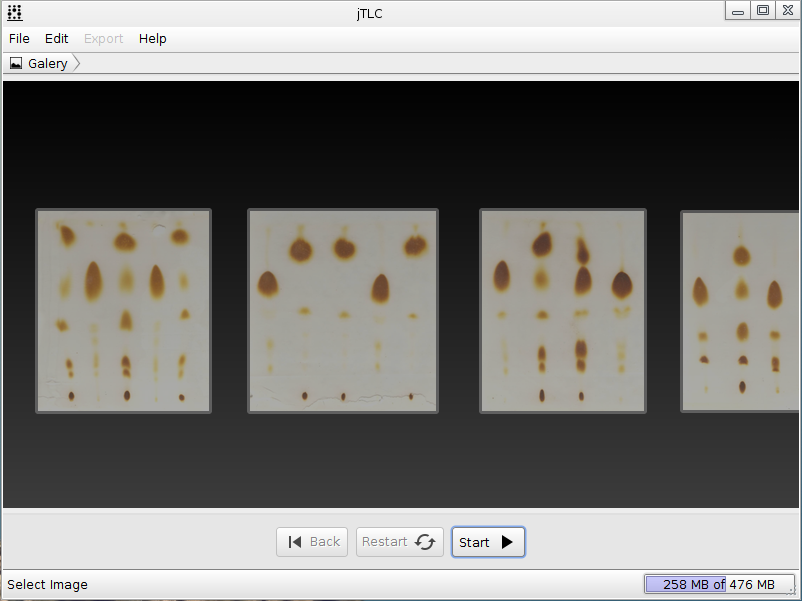
\includegraphics[width=385px]{imagenes/gallery}
	\centering
	\vspace{-0.4cm}
	\caption{Projects gallery.}
	\label{fig:gallery}
	\vspace{-0.25cm}
\end{figure}
\newpage

\section{Edit Project}
To edit the data of current project use the option \emph{Edit project} in the menu \emph{Edit}, a \emph{Edit project data} dialog will be shown where the user can change the project title, description and dates. Use the button \emph{Accept} to save the current values or \emph{Cancel} to abort.
\begin{figure}[H]
	\vspace{0cm}
	\centering
	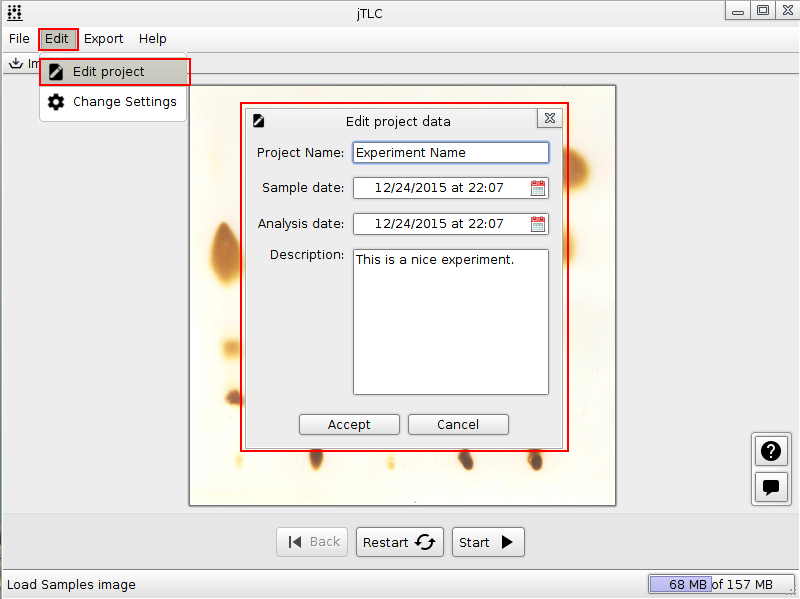
\includegraphics[width=385px]{imagenes/edit_project}
	\centering
	\vspace{-0.4cm}
	\caption{Edit project data.}
	\label{fig:edit_project}
	\vspace{-0.25cm}
\end{figure}
\newpage

\section{Save Project}
To save current project use the option \emph{Overwrite Project}, if exist a previous version (file) of project, or the option \emph{Save Project as...} if it's a new project, in the \emph{File} menu. The option \emph{Overwrite Project} will overwrite the current project file with the new values and data. The option \emph{Save project as...} display a \emph{File Chooser} dialog where you can select a Folder and a File where the project data will be written. Select a File to overwrite/replace or write a new file name (by default it's the project title) and then press the button \emph{Save} to accept or \emph{Cancel} to abort.

\begin{figure}[H]
	\vspace{0cm}
	\centering
	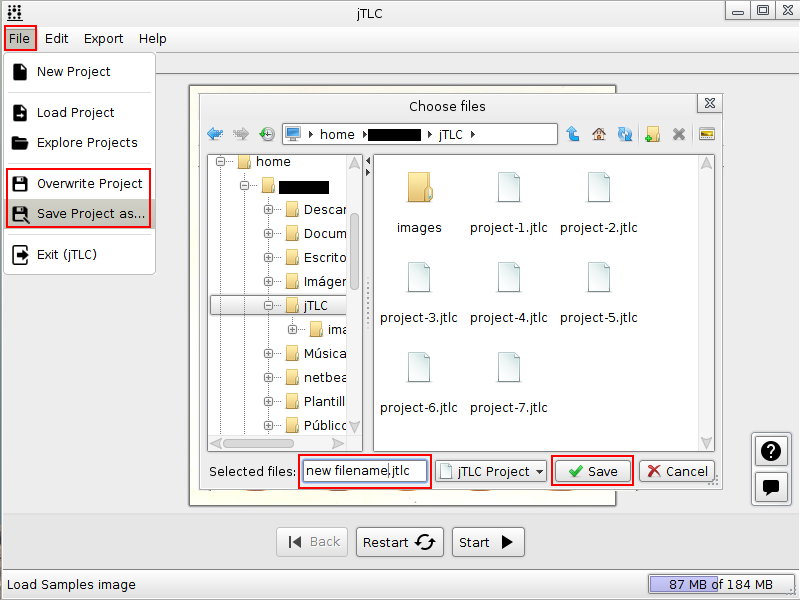
\includegraphics[width=385px]{imagenes/save_project}
	\centering
	\vspace{-0.4cm}
	\caption{Save current project.}
	\label{fig:save_project}
	\vspace{-0.25cm}
\end{figure}
\newpage

\chapter{Samples Analysis}
\section{Image Load}
El primer paso para el análisis de una muestra es cargar la im\'agen. Dicha tarea se puede realizar de dos formas. La primera es haciendo uso de la funci\'on \emph{drag & drop}, que le permitir\'a al usuario utilizar el mouse para arrastras un archivo hacia la zona central rodeada por l\'ineas de puntos. La segunda opci\'on que permite la carga del archivo es hacer click sobre la zona central rodeada por l\'ineas de puntos, lo que a continuaci\'on abrir\'a una ventana que permite la selecci\'on de archivos a trav\'es de la b\'usqueda de archivos entre carpetas.
\begin{figure}[H]
	\vspace{0cm}
	\centering
	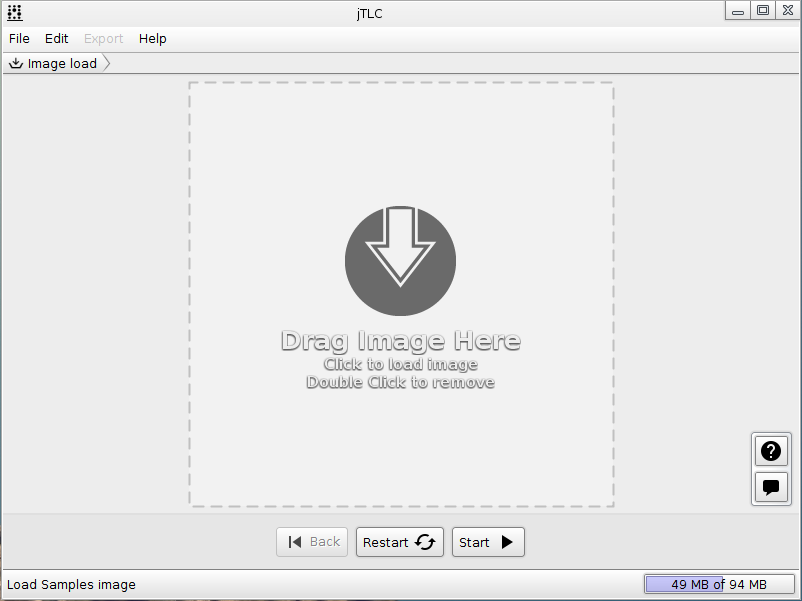
\includegraphics[width=385px]{imagenes/drop}
	\centering
	\vspace{-0.4cm}
	\caption{Load experiment image.}
	\label{fig:image_load}
	\vspace{-0.25cm}
\end{figure}

\section{Image Crop}
El corte de im\'agenes se realiza utilizando dos sliders, uno vertical y otro horizontal, que permitir\'an correr las líneas de corte desde los m\'argenes laterales y los m\'argenes superior e inferior.
\begin{figure}[H]
	\vspace{0cm}
	\centering
	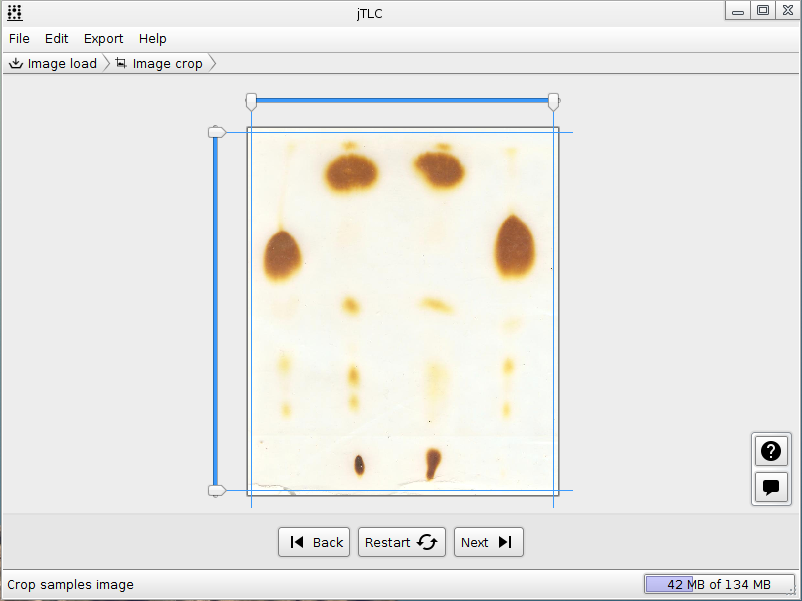
\includegraphics[width=385px]{imagenes/crop}
	\centering
	\vspace{-0.4cm}
	\caption{Crop samples image.}
	\label{fig:image_cut}
	\vspace{-0.25cm}
\end{figure}

\section{Image Rotation}
Esta secci\'on le permite al usuario rotar la im\'agen. Se ofrecen las opciones: \emph{\'angulo de rotaci\'on}, el usuario selecciona el \'angulo preciso a rotar; \emph{girar a la derecha}, gira la im\'agen 90 grados a la derecha; \emph{girar a la izquierda}, gira la im\'agen 90 grados a la izquierda; \emph{invertir verticalmente}, invierte la im\'agen en sentido vertical; \emph{invertir horizontalmente}, invierte la im\'agen en sentido horizontal.
\begin{figure}[H]
	\vspace{0cm}
	\centering
	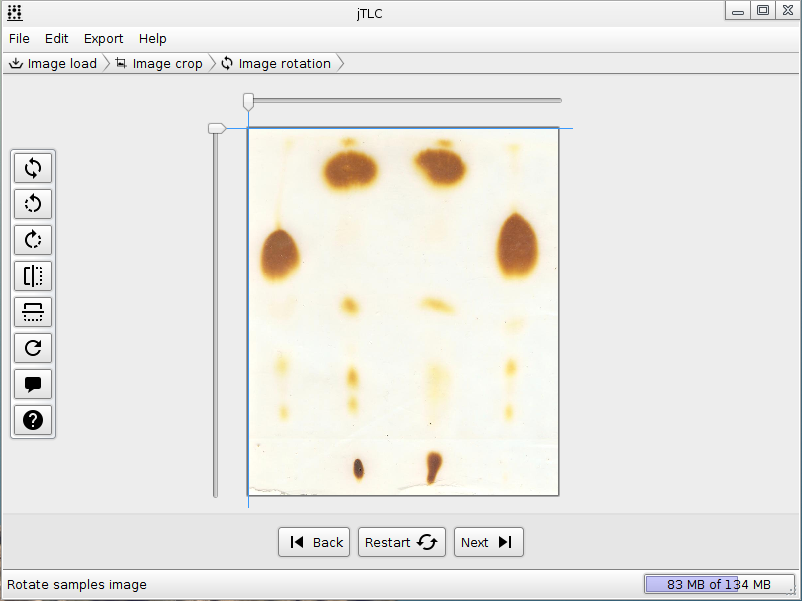
\includegraphics[width=385px]{imagenes/rotate}
	\centering
	\vspace{-0.4cm}
	\caption{Rotate and flip samples image.}
	\label{fig:image_rot}
	\vspace{-0.25cm}
\end{figure}

\section{Samples Selection}
En esta etapa del proceso el usuario puede seleccionar con un slider las muestras que ser\'an analizadas. Para poder agregar una muestra se debe realizar doble click sobre el slider, mientras que para eliminarlo se debe oprimir el bot\'on \emph{suprimir} del teclado.
\begin{figure}[H]
	\vspace{0cm}
	\centering
	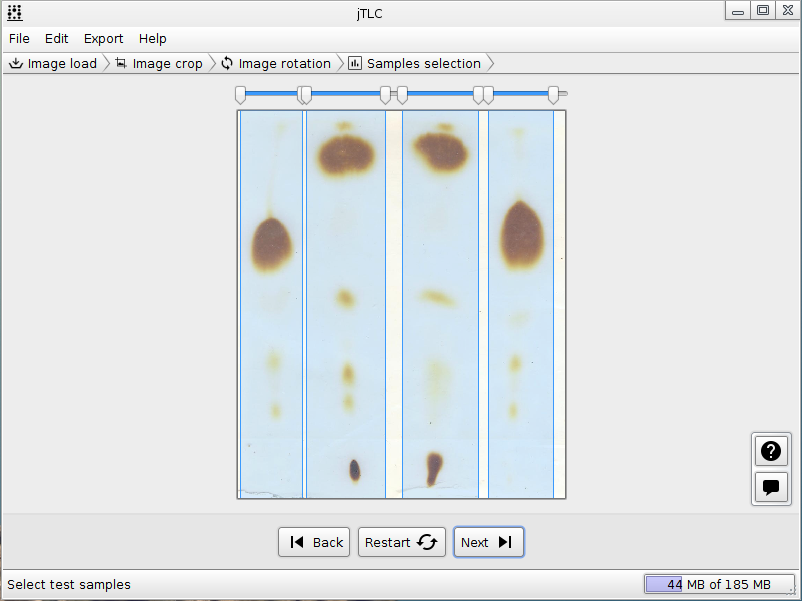
\includegraphics[width=385px]{imagenes/selection}
	\centering
	\vspace{-0.4cm}
	\caption{Individual samples selection.}
	\label{fig:image_samples_selection}
	\vspace{-0.25cm}
\end{figure}

\section{Samples Special Points}
La selecci\'on de puntos especiales puede realizarse de dos formas. La primera es individualmente, mientras que la segunda permite sincronizar la ubicación de los puntos especiales activando la opción para ello debajo de las muestras que se desean alinear conjuntamente.
\begin{figure}[H]
	\vspace{0cm}
	\centering
	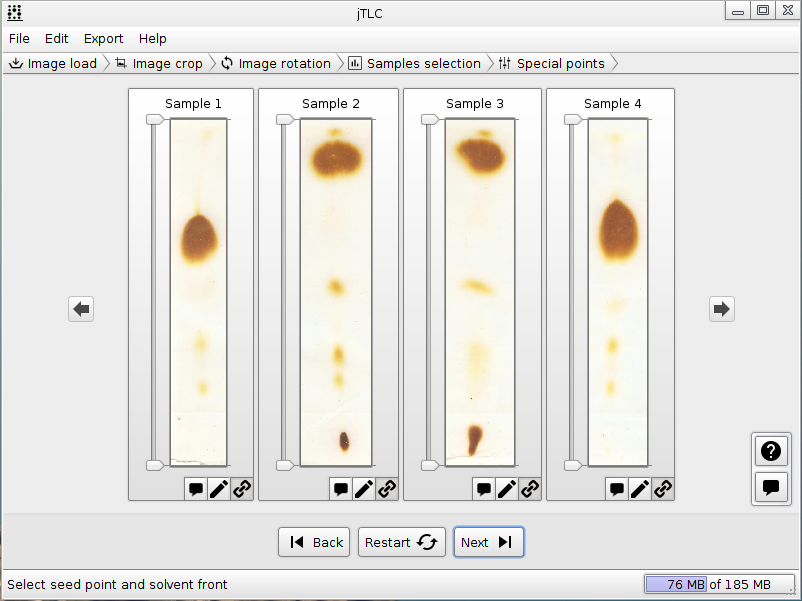
\includegraphics[width=385px]{imagenes/points}
	\centering
	\vspace{-0.4cm}
	\caption{Samples data and special points selection.}
	\label{fig:image_samples_special_points}
	\vspace{-0.25cm}
\end{figure}

\section{Samples Peaks Selection}
Uno de los pasos finales es la selecci\'on de picos para cada muestra. La ventana se divide en pesta\~nas, una por cada muestra, para exhibir los picos hallados y el usuario a la vez puede modificar o agregar picos de forma s\'imil al momento de seleccionar las muestras. Se ofrece un slider sobre la gráfica y otro al costado de la muestra, ambos representan en paralelo el mismo sector de la muestra y es posible agregar un \'area a partir de cualquier de las dos opciones.
\begin{figure}[H]
	\vspace{0cm}
	\centering
	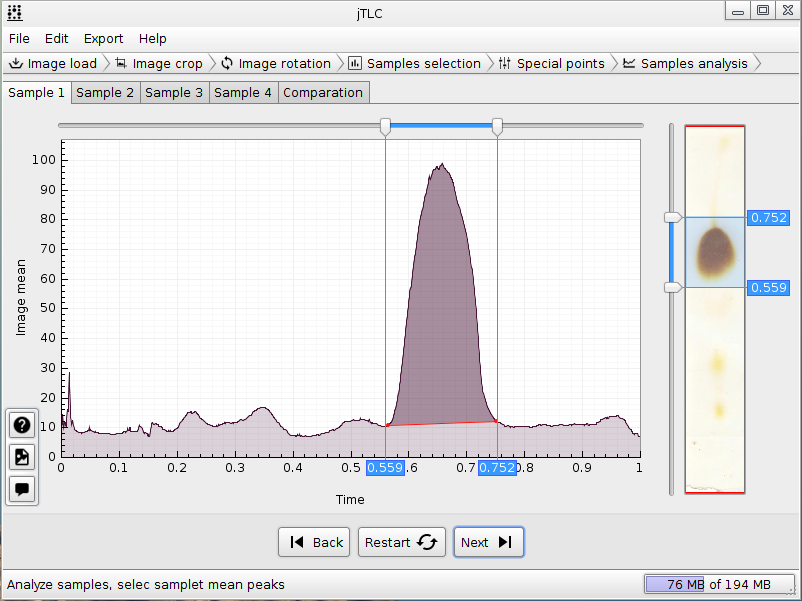
\includegraphics[width=385px]{imagenes/analysis}
	\centering
	\vspace{-0.4cm}
	\caption{Individual samples peaks selection.}
	\label{fig:image_samples_peaks}
	\vspace{-0.25cm}
\end{figure}

\section{Samples Comparation}
Al final de la lista de pesta\~nas se puede ver una que dice \emph{comparaci\'on} que muestra todas las gr\'aficas en una con colores diferentes para cada una, dicho color es modificable e incluso es posible quitar el relleno transparente, o bien seleccionar cu\'ales muestras ver en la comparaci\'on.
\begin{figure}[H]
	\vspace{0cm}
	\centering
	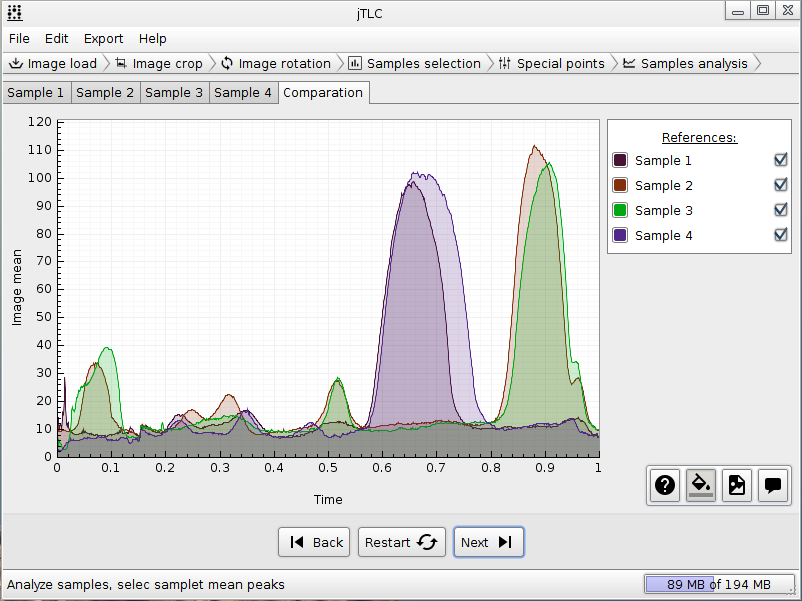
\includegraphics[width=385px]{imagenes/comparation}
	\centering
	\vspace{-0.4cm}
	\caption{Experiment samples mean comparation.}
	\label{fig:image_samples_comparation}
	\vspace{-0.25cm}
\end{figure}

\section{Analysis Results}
De forma an\'aloga a la fase anterior, se muestran los resultados para cada muestra con informaci\'on del an\'alisis realizado en cada pico: l\'imites, m\'aximo, m\'inimo, altura, superficie, superficie relativa y l\'inea  base. Adem\'as se ofrece la opci\'on para exportar la im\'agen de la gr\'afica.
\begin{figure}[H]
	\vspace{0cm}
	\centering
	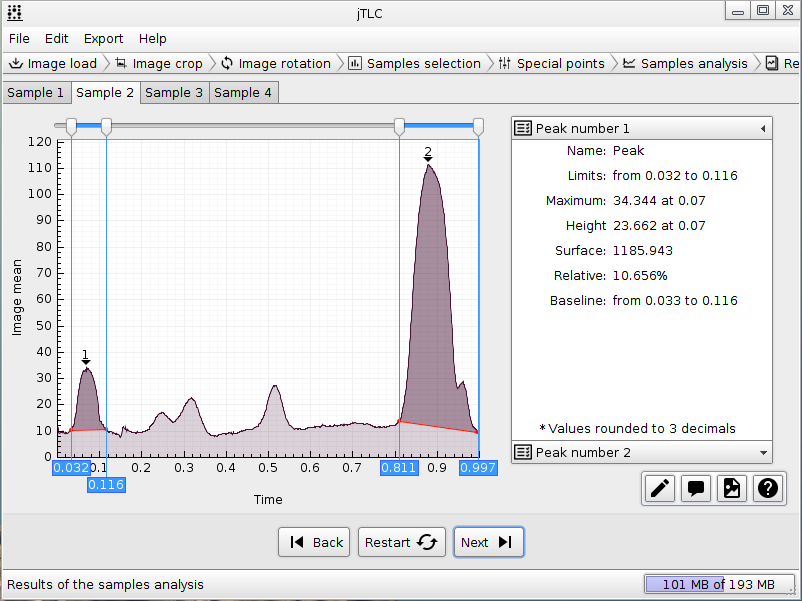
\includegraphics[width=385px]{imagenes/peaks}
	\centering
	\vspace{-0.4cm}
	\caption{Samples peaks analysis results.}
	\label{fig:image_analysis_results}
	\vspace{-0.25cm}
\end{figure}

\section{Analysis Reports}
Nuevamente, haciendo uso de la ventana con pesta\~nas, se muestra la informaci\'on de cada muestra en forma de reporte con toda la informaci\'on, im\'agenes iniciales y procesadas. Tambi\'en se muestra, en al primer pesta\~na, informaci\'on general del proyecto junto con la im\'agen que contiene a todas las muestras.
\begin{figure}[H]
	\vspace{0cm}
	\centering
	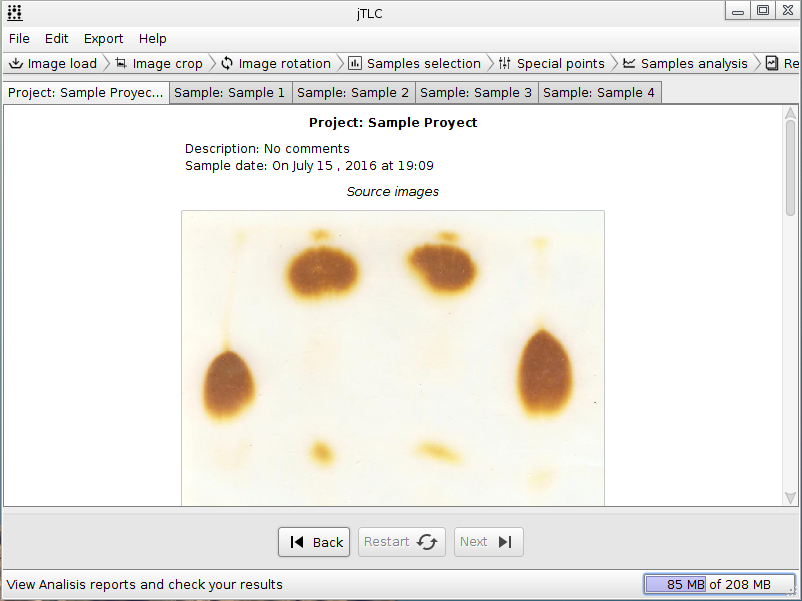
\includegraphics[width=385px]{imagenes/reports}
	\centering
	\vspace{-0.4cm}
	\caption{Samples analysis reports.}
	\label{fig:image_analysis_reports}
	\vspace{-0.25cm}
\end{figure}

\chapter{Data Export}
\section{Export images}
Para exportar las im\'agenes que se trabajaron en la aplicaci\'on se debe seleccionar la opción \emph{exportar}, luego, entre la listas de acciones que ofrece el men\'u emergente se debe seleccionar \emph{Im\'agenes originales} lo que ofrecer\'a como resultado son las im\'agenes iniciales: la im\'agen inicial que contiene toda la muestra y las muestras individuales. Cada im\'agen luego de ser seleccionada se muestra en una ventana emergente con la posibilidad de redimensionar la misma antes de elegir cu\'al es el directorio en el que se desea guardar la im\'agen.
Otra opci\'on que ofrece el men\'u \emph{exportar}, es \emph{Im\'agenes procesadas}, lo cual ofrece las mismas im\'agenes de la primer opci\'on pero con el proceso de recorte y giro de la im\'agen aplicado.

\section{Export reports}
Para exportar informaci\'on del proyecto se debe seleccionar la opci\'on \emph{exportar} y dentro del men\'u de opciones elegir \emph{Reportes}. Las opciones que en este punto se ofrecen son para exportar datos del proyecto o bien de las muestras individuales. A la vez, sobre cada opci\'on para exportar se permite decidir sobre el formato del documento a exportar: PDF, ODT, HTML o CSV. 
La opci\'on para exportar el proyecto, ofrece la informaci\'on completa sobre el mismo. Es decir, im\'agen original y modificada, comentarios \'angulo de correcci\'on sobre giro, puntos de corte del recorte de la im\'agen y puntos de corte para separar las muestras. A continuaci\'on, se muestra consecutivamente informaci\'on sobre cada muestra individual (dichos datos son los que se pueden exportar individualmente). Los datos que se exhiben en cada muestra individual son las im\'agenes originales, im\'agenes procesadas, puntos de l\'imite, punto de siembra, frente solvente, im\'agen de media y picos de la muestra,superficie absoluta, comentarios sobre cada paso del proyecto, enumeraci\'on de picos: pisici\'on, l\'imites, m\'aximo, m\'inimo, altura, superficie absoluta, superficie relativa y l\'inea base.

\section{Export data}
\subsection{Export mean}
Para exportar informaci\'on sobre la media de cada muestra se debe utilizar la opci\'on \emph{exportar}, luego seleccionar \emph{media} y la muestra de la cual se quiere extraer la informaci\'on; paso a seguir, se descargar\'a un archivo de texto con los datos solicitados.

\subsection{Export plain data}
Esta opci\'on permite exportar, en documentos de texto plano, informaci\'on sobre el proyecto con nombre, comentarios y datos extras (fechas y modificaciones a la im\'agen original). Cuando se selecciona una muestra particular se muestra informaci\'on sobre ubicaci\'on de puntos especiales, comentarios, l\'imites, superficie, altura, m\'aximo, m\'inimo y l\'inea de base por pico.